\chapter{Additional Data A}

\section{Existence of an Additional Root in Cubic Functions via the Intermediate Value Theorem}

\textbf{Theorem:} Let \( f(x) = ax^3 + bx^2 + cx + d \) be a cubic function, where \( a, b, c, d \in \mathbb{R} \) and \( a \neq 0 \). If \( x_1 \) and \( x_2 \) are two distinct roots of \( f(x) \), there exists at least one other root \( x_3 \) of \( f(x) \).

\textbf{Proof:}

\begin{enumerate}
	\item \textit{Cubic Function}: A cubic function is defined as \( f(x) = ax^3 + bx^2 + cx + d \), which is a polynomial of degree 3, and thus continuous over \(\mathbb{R}\).
	
	\item \textit{Known Roots}: Assume \( x_1 \) and \( x_2 \) are two distinct roots of \( f(x) \), i.e., \( f(x_1) = f(x_2) = 0 \).
	
	\item \textit{Intermediate Value Theorem (IVT)}: The IVT states that for any continuous function \( g \) on an interval \([a, b]\), if \( g(a) \) and \( g(b) \) have opposite signs, there is at least one \( c \) in \((a, b)\) such that \( g(c) = 0 \).
	
	\item \textit{Application to Cubic Function}: By the nature of cubic functions, they must change direction at least once between two roots. This implies the function will either attain a local maximum or minimum between \( x_1 \) and \( x_2 \).
	
	\item \textit{Existence of Third Root}: If the local extremum is above or below the x-axis, the function must cross the x-axis to change direction, implying the existence of another root \( x_3 \) in the interval \((x_1, x_2)\).
	
	\item \textit{Conclusion}: Therefore, by drawing a straight line through \( (x_1, 0) \) and \( (x_2, 0) \), this line will intersect the graph of \( f(x) \) at least at one other point, indicating the existence of another root \( x_3 \).
\end{enumerate}

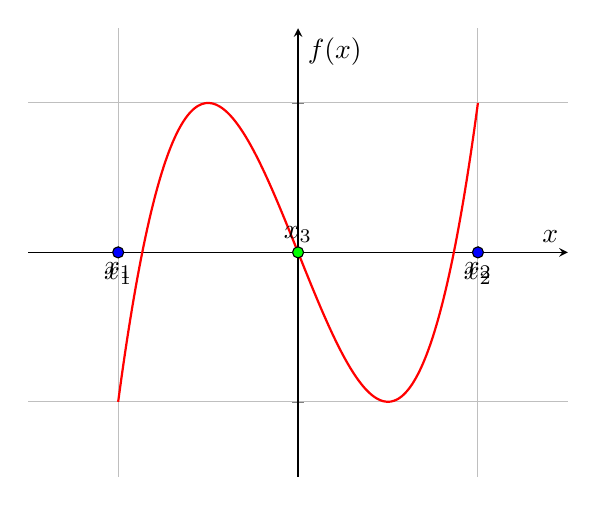
\begin{tikzpicture}
	\begin{axis}[
		xlabel={$x$},
		ylabel={$f(x)$},
		axis lines=middle,
		xmin=-3, xmax=3,
		ymin=-3, ymax=3,
		grid=both,
		xtick={-2, 0, 2},
		ytick={-2, 0, 2},
		xticklabels={$x_1$, $0$, $x_2$},
		yticklabels={,,}
		]
		
		% Cubic function
		\addplot[smooth, thick, red] expression[domain=-2:2, samples=100]{x^3 - 3*x};
		
		% Dots at roots
		\addplot[only marks, mark=*, mark options={fill=blue}] coordinates {(-2,0) (2,0)};
		
		% Optional: Add a point for the third root
		\addplot[only marks, mark=*, mark options={fill=green}] coordinates {(0,0)};
		
		% Labels for the roots
		\node[below] at (axis cs:-2,0) {$x_1$};
		\node[below] at (axis cs: 2,0) {$x_2$};
		\node[above] at (axis cs: 0,0) {$x_3$};
		
	\end{axis}
\end{tikzpicture}

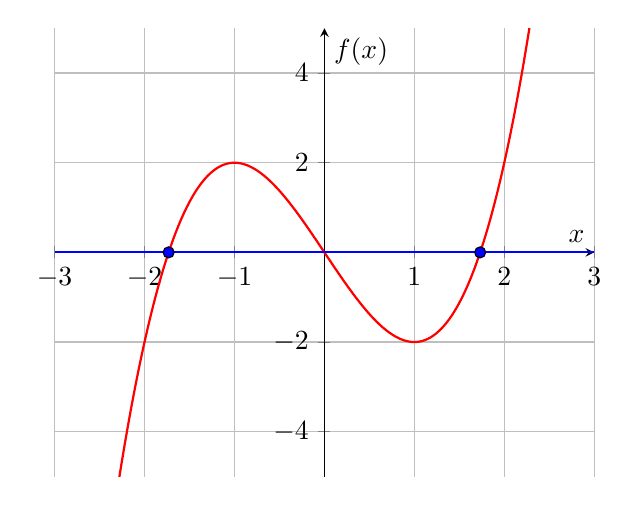
\begin{tikzpicture}
	\begin{axis}[
		xlabel={$x$},
		ylabel={$f(x)$},
		axis lines=middle,
		xmin=-3, xmax=3,
		ymin=-5, ymax=5,
		grid=both
		]
		
		% Define a cubic function
		\addplot[smooth, thick, red, domain=-3:3, samples=100] {x^3 - 3*x};
		
		% Mark the known roots
		\addplot[only marks, mark=*, mark options={fill=blue}] coordinates {(-sqrt(3),0) (sqrt(3),0)};
		
		% Draw a straight line through the two known roots
		\addplot[thick, blue, domain=-3:3] {0};
		
%		% Label for roots and potential third root
%		\node[below] at (axis cs:-sqrt(3),0) {$x_1$};
%		\node[below] at (axis cs: sqrt(3),0) {$x_2$};
%		\node[above] at (axis cs: 0,0) {Possible $x_3$};
		
	\end{axis}
\end{tikzpicture}

\begin{tikzpicture}[scale=0.5, >=Stealth]
	
	% Define the range for drawing
	\foreach \x in {-5,...,5} {
		\foreach \y in {-5,...,5} {
			% Place a dot at each point
			\node[draw,circle,inner sep=1pt,fill] at (\x,\y) {};
		}
	}
	
	% Draw vectors
	\draw[thick,->] (-4,-3) -- (4,-1) node[midway, below] {$\mathbf{v}_1$};
	\draw[thick,->] (-4,-3) -- (-3,1) node[midway, above] {$\mathbf{v}_2$};
	
	% Optional: Draw coordinate axes
	\draw[thin,->] (-6,0) -- (6,0) node[right] {$x$};
	\draw[thin,->] (0,-6) -- (0,6) node[above] {$y$};
	
\end{tikzpicture}

% Appendix A content
